\documentclass[12pt]{article}

\usepackage[a4paper, left=3.17cm, right=3.17cm, top=2.54cm, bottom=2.54cm]{geometry}
\usepackage[T1]{fontenc}
\usepackage{mathptmx}
\usepackage{amsmath}
\usepackage{amsfonts}
\usepackage{chemformula}
\usepackage{cite}
\usepackage[colorlinks, linkcolor=black, anchorcolor=black, citecolor=black]{hyperref}
\usepackage{graphicx}
\usepackage{fancyhdr}
\usepackage{enumitem}
\usepackage{listings}
\usepackage{setspace}
\usepackage[a4paper]{geometry}
\usepackage[ruled]{algorithm2e}

\geometry{left=2cm, right=2cm, top=3cm, bottom=2.5cm}

\setlength{\parskip}{0.5em}
\title{Strip Packing \\ \bigskip \large Project6\ \ Report\ \ by\ \ Group1}
\author{Guo Jiahao \\ Wu Yihang \\ Sun Xinjie}

\lstset{
    columns=fixed,       
    numbers=left,                                        % 在左侧显示行号
    numberstyle=\tiny\color{gray},                       % 设定行号格式
    frame=none,                                          % 不显示背景边框
    backgroundcolor=\color[RGB]{245,245,244},            % 设定背景颜色
    keywordstyle=\color[RGB]{40,40,255},                 % 设定关键字颜色
    numberstyle=\tiny,keywordstyle=\color{blue!70},
    commentstyle=\color{red!50!green!50!blue!50},frame=shadowbox,
    rulesepcolor=\color{red!20!green!20!blue!20},basicstyle=\ttfamily,
    stringstyle=\rmfamily\slshape\color[RGB]{128,0,0},   % 设置字符串格式
    showstringspaces=false,                              % 不显示字符串中的空格
    language=C++,                                        % 设置语言
    }

\pagestyle{fancy}
\fancyhf{}
\cfoot{\thepage}
\fancyhead[C]{Advanced Data Structure and Algorithm Analysis\ \ \ \ Project6  Report\ \ \ \ Group1}
\begin{document}

\begin{titlepage}
	\newcommand{\HRule}{\rule{\linewidth}{0.5mm}}
	\begin{figure}
        \flushleft
        
\includegraphics[scale=0.4]{0.png}
    \end{figure}
    \center 
	\quad\\[1.5cm]
	\textsl{\Large Zhejiang University }\\[0.5cm] 
	\textsl{\large College of Computer Science and Technology}\\[0.5cm] 
	\makeatletter
	\HRule \\[0.4cm]
	{ \huge \bfseries \@title}\\[0.4cm] 
	\HRule \\[1.5cm]
	\begin{minipage}{0.4\textwidth}
		\begin{flushleft} \Large
			\emph{Author:}\\
			\@author 
		\end{flushleft}
	\end{minipage}
	~
	\begin{minipage}{0.4\textwidth}
		\begin{flushright} \Large
			\emph{Supervisor:} \\
			\textup{Mao Yuchen}
		\end{flushright}
	\end{minipage}\\[3cm]
	\makeatother
	\begin{flushleft}
        \Large
        \textbf{Abstract:}

    \end{flushleft}
    {\large An Assignment submitted for the ZJU:}\\[0.5cm]
	{\large {21120491\ \ Advanced Data Structure and Algorithm Analysis}}\\[0.5cm]
	{\large \today}\\[2cm] 
	\vfill 
\end{titlepage}
    
    \section{Introduction of the Project}
    In this project, we need to solve the strip packing problem.
    The strip packing problem is a 2-dimensional geometric minimization problem.
    Given a set of axis-aligned rectangles and a strip of bounded width and infinite height,
    determine an overlapping-free packing of the rectangles into the strip minimizing its height.
    We may assume that the width of any rectangle is no more than the width of the bin,
    and we are not allowed to rotate the rectangles, and that the rectangles should not overlap.

    Note that we need to implement at least two polynomial-time approximation algorithms for this problem.
    We must generate test cases of different sizes with different distributions of widths and heights,
    compare and analysis the solution quality and the running time of the two algorithms on these test cases. 

    \section{Introduction of the Algorithms}
    \subsection{Next Fit(NF)}
    We first discuss the simplest method to solve this problem which called next fit algorithm.
    In this algorithm, We place the rectangles one by one.
    When the bottom edge of the next rectangle cannot be placed at the same height as the previous rectangle,
    we cover the "cover" of the previous layer, that is,
    place the bottom edge of the next rectangle on the height of the top of the highest rectangle on the current layer.
    Pseudo code is shown below:
    \begin{algorithm}
        \caption{Next Fit(NF)}
        \LinesNumbered
        \KwIn{width \emph{w} and height \emph{h} of input rectangles}
        let \emph{h = 0}\;
        \For{Rectangle R = (w, h)\textup{in the sequence}}{
            Try to fit the rectangle onto the current open shelf\;
            \If{\textup{It does not fit}}{
                close the current shelf and open a new one\;
                \emph{h = h + }max height of the previous layer\;
            }
        }
    \end{algorithm}

    \subsection{First Fit(FF)}
    Then we discuss the first fit algorithm, which is the first optimized 
    algorithm we discuss today. This time we don't cover the "cover" immediately 
    after we can't put the next rectangle at the previous level. This time if the next 
    rectangle can be put into the interval of any previous layer, we put this rectangle 
    into the first layer that satisfies. Pseudo code is shown below:
    \begin{algorithm}
        \caption{First Fit(FF)}
        \LinesNumbered
        \KwIn{width \emph{w} and height \emph{h} of input rectangles}
        let \emph{h = 0}\;
        \For{Rectangle R = (w, h)\textup{in the sequence}}{
            Using bisection method to find the first layer that can fit the rectangle\;
            \If{\textup{No previous layer fit}}{
                close the current shelf and open a new one\;
                \emph{h = h + }height of the rectangle\;
            }
        }
    \end{algorithm}

    \subsection{Best Width Fit(BWF)}
    Now we need to discuss the second optimized algorithm which is 
    similar to the first fit algorithm, but this time we don't put 
    the next rectangle to the first layer that fit the rectangle but the best 
    layer where best means the it has the smallest interval that 
    fit the new rectangle. Pseudo code is shown below:
    \begin{algorithm}
        \caption{Best Width Fit(BWF or BF briefly)}
        \LinesNumbered
        \KwIn{width \emph{w} and height \emph{h} of input rectangles}
        let \emph{h = 0}\;
        \For{Rectangle R = (w, h)\textup{in the sequence}}{
            Using balanced tree to find the best fit layer\;
            \If{\textup{No previous layer fit}}{
                close the current shelf and open a new one\;
                \emph{h = h + }height of the rectangle\;
            }
        }
    \end{algorithm}

    Let’s look at an example to understand thoroughly how the algorithms works. When the width
    required is 10 and the following rectangles are to be placed: 

    Rectangle (5, 6) - Rectangle (3, 5) - Rectangle (9, 4) - Rectangle (10, 3) - Rectangle (1, 2) -
    Rectangle (2, 1)

    \begin{figure}[h]
        \centering
        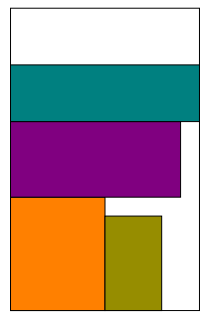
\includegraphics[scale=0.4]{1.png}
        \caption{After inserting the first four rectangles}
    \end{figure}

    \begin{figure}[h]
        \centering
        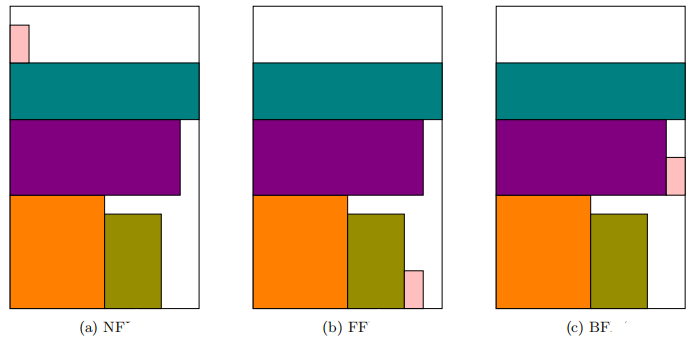
\includegraphics[scale=0.5]{2.png}
        \caption{After inserting the fifth rectangle}
    \end{figure}

    \begin{figure}[h]
        \centering
        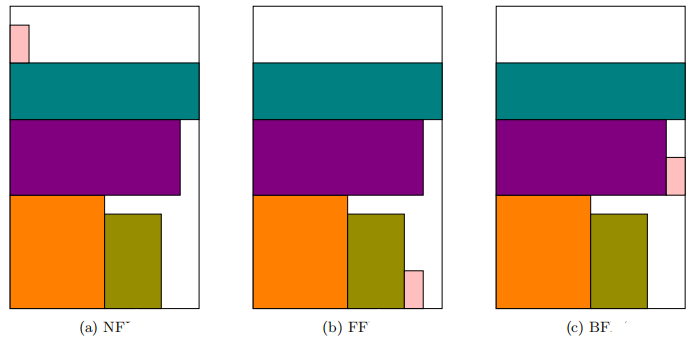
\includegraphics[scale=0.5]{2.png}
        \caption{After inserting the sixth rectangle}
    \end{figure}

    As is shown in 1, the three algorithms yield the same result when the rectangles are inserted 
    in specific way. While the empty space for the current level is not enough, first fit and best fit use 
    different way to manage it rather than creating a new level, as is shown in 2b and 2c. The way 
    for best fit is cleverer than first fit since the empty space is managed better, as is shown in 3c.

    \section{Algorithm Analysis}
    \subsection{Running time}
    \subsubsection{Next Fit}
    It's easy to see that we only need \emph{O}(\emph{n}) time where n 
    is the number of inout rectangles(the same in the following sections) because for every input rectangle, 
    we only need to judge if it can be put in the current layer in constant 
    time, so the total time is linear.

    \subsubsection{First Fit}
    Because for every input rectangle, we need to find the previous layers to 
    determine where to put. If we use linear scan to find the first fit position, 
    $O(n)$ time is needed. If we use bisection method, we only need 
    \emph{O}(log\emph{n}) time to implement this algorithm.

    \subsubsection{Best Width Fit}
    Because for every input rectangle, we need to find the previous layers to 
    determine where to put. If we use linear scan to find the best fit position, 
    $O(n)$ time is needed. If we use balanced tree to find the proper position, we only need 
    \emph{O}(log\emph{n}) time to implement this algorithm.

    \subsection{Approximation rate}
    Let’s denote the optimal result as \emph{OPT}, the sum of areas of all rectangles \emph{A}, the result of 
    NF, FF and BWF \emph{NF}, \emph{FF} and \emph{BWF}respectively. We have implied in the example that
    $$OPT \le BWF \le FF \le NF$$
    For the convenience of our proof, assume all width are normalized to the required width, 
    i.e set the required width to 1 and all rectangles has width smaller than 1 for convenience. 
    First of all, we would estimate the approximation ratio of NF as an upperbound of all the algorithms[1].

    \textbf{Theorem 1.} $NF \le 2OPT + h_{max}$ where $h_{max}$ is the maximun height of 
    all the input rectangles.

    \emph{Proof.} Denote the height of level \emph{i} $H_{i}$, then
    $$NF = \sum_{i}H_{i}$$
    Because the next level is generated as long as the first rectangle in the next level is not compactible 
    with the current level, we have
    $$A_{i} + A_{i+1} \ge H_{i+1}$$
    where $A_{i}$ denotes the total area of the rectangles in level \emph{i}. Thus:
    $$NF = H_{1} + \sum_{i=2}^{n}H_{i} \le H_{1} + 2A \le H_{1} + 2OPT$$
    Then we are to show a result about the upperbound of the FF algorithm, which is 
    more more complicated.

    \textbf{Theorem 2.} $FF \le 1.7OPT + h_{max}$ where $h_{max}$ is the maximun height of 
    all the input rectangles.

    Proof of the above theorem[1] is omitted here for clarity. BF approximation ratio
    is hard to estimate, with no related works found.
    \section{Experiment and Result}
    \begin{table}[h]
        \centering
		\begin{tabular}{l l l l l}
			
			\textbf{Operation} & \textbf{Binary heap} & \textbf{Leftist heap} & \textbf{Binomial heap} & \textbf{Fibonacci heap}\\
			
			Make heap    & \emph{O}(\emph{n}) & \emph{O}(\emph{n}) & \emph{O}(\emph{n}) & \emph{O}(\emph{n})\\
			Find min     & \emph{O}(1)        & \emph{O}(1)        & \emph{O}(1)        & \emph{O}(1)\\
			Insert       & \emph{O}(log\emph{n}) & \emph{O}(log\emph{n}) & \emph{O}(log\emph{n}) & \emph{O}(1)\\
            Delete min   & \emph{O}(log\emph{n}) & \emph{O}(log\emph{n}) & \emph{O}(log\emph{n}) & \emph{O}(log\emph{n})\\
            Merge        & \emph{O}(\emph{n}) & \emph{O}(log\emph{n}) & \emph{O}(log\emph{n}) & \emph{O}(1)\\
            Delete       & \emph{O}(log\emph{n}) & \emph{O}(log\emph{n}) & \emph{O}(log\emph{n}) & \emph{O}(log\emph{n})\\
            Decrese key  & \emph{O}(log\emph{n}) & \emph{O}(log\emph{n}) & \emph{O}(log\emph{n}) & \emph{O}(1)
		\end{tabular}
		\caption{Running times of all operations of different heaps}
	\end{table}
    \section{Discussion and Conclusion}
    
    \section{References}
    [1] \emph{Performance Bounds for Level-Oriented Two-Dimensional Packing Algorithms}, 
    E. G. Coffman, Jr., M. R. Garey, D. S. Johnson, and R. E. Tarjan, SIAM Journal on Computing 1980 9:4, 808-826
\end{document}